%\section{Method} \label{sec:method}
In this chapter the general workflow used throughout the entire project is described. Furthermore we present how the collaboration was performed and which strategies we used. 
%% NOTE TO SELF: The level of abstraction is focused on describing the process and discuss what could have been done differently.

\section{Workflow} \label{sec:workflow}
In our design of a policy engine, we decided to use an iterative design approach, both for the frontend and backend. Using this approach we were able to continuously evaluate both the concept and our software. We have done a lot of informal testing throughout the complete project. The goal has been to continuously test and optimize the software, learn about the stability and performance, and finally to adjust the implementation according to these findings. 

An iterative design approach is commonly used for the frontend design. This allows designers to identify any usability issues that may arise in the user interface before it is put into wide use. Even the best usability experts cannot design perfect user interfaces in a single attempt, so a usability engineering life cycle should be built around the concept of iteration \cite{Nielsen1993}.

The figure below (fig. \ref{fig:workflow}) illustrates the different iterations, phases and stages of our project.

\begin{figure}[ht]
\centering
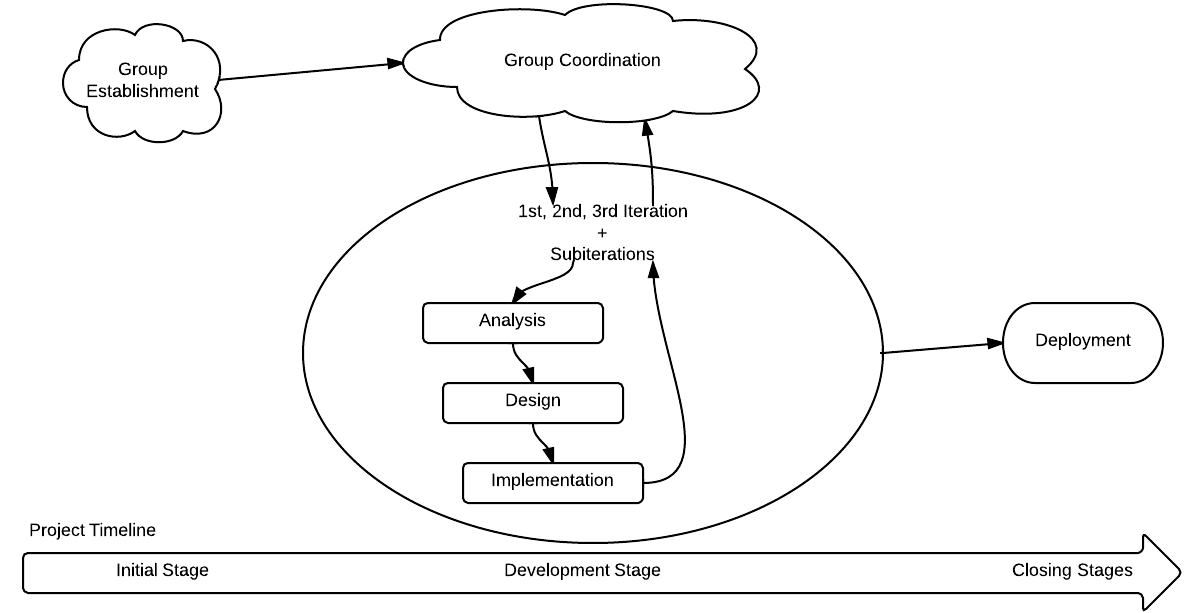
\includegraphics[width=\columnwidth]{images/workflow.png}
\caption{A generalized view of our workflow process}
\label{fig:workflow}
\end{figure}

Each of these illustrated elements were important for the process and contains all valuable information. The figure contains a timeline, which chronologically shows how the project evolved. The project went through three overall phases. These are the ``Initial Stage'', ``Development Stage'' and ``Closing Stage''.

\subsection{Stages} \label{subsec:stages}
\subsubsection{Initial Stage}
Before kicking off the project and delve into the actual development, we needed to figure out how to handle the group as \textit{one} collaborating team. This part was of high importance due to the fact that we, as students from two different continents, did not know each other at all. The task was also complicated by this. One could presume that in a normal work setting at least the different roles in the team would already have been settled. Some is hired to do the backend (developer) and others others to manage the project (project manager). We needed a specific initial stage to cover this part of getting to know each other, figure out roles and knowledge areas. This was internally known as the ``Initial Stage''. This created the necessary basis to work from and we could start to move the project in the right direction. %begin to analyse and develop according to the requirements.
\subsubsection{Development Stage}
During the development stage several iterations of analysis, design and implementation were executed. As the figure shows, the repetitive phases in the development stage is an iterative process. Even though we were through this loop multiple times, we will only describe the three major iterations, in the section below. These iterations are coherent with the project plan and follows our general approach to the project. All of the three iterations contains multiple inclusive \textemdash by assessing the artefact\textemdash iterations. Describing each iteration in detail would be a some what cumbersome process.

The reasoning for choosing three major iterations was to accommodate the overall deadlines for the project. Each deadline requested different material containing information about different levels of the project. The first deadline was focused on the requirements and motivation. The second delivery focused on related work and model. Third delivery's focus was on the actual product and its code. These deadlines were a part of our overall project plan and thus led to having three overall milestones and one deadline.

The development stage contains a group coordination phase. The coordination is reached multiple times throughout the major iterations. During this phase important topics were covered, such as sharing status, separation and distribution of tasks, figure out how to proceed, discuss upcoming challenges and the likes.

\subsubsection{Deployment Stage}
The deployment stage was considered the simplest and easiest to handle stage of our process. Upon reaching agreement that the development was finalized, the product was deployed to our server. This concluded our work on the product and finalized the development.

\subsection{Iterations} \label{subsec:iterations}

\subsubsection{First Iteration}
Our focus during the first iteration was to get the group work to flow and figure out how to handle the data services provided by the Danish university. Most of the iteration was related to get to know each other and figure out how to move the project forward. The artefacts produced here was very low level, such as diagrams of the group members programming skills, use case diagrams, first thoughts of domain model, early prototypes of the frontend interface and early implementations of the data services.

It was difficult to really push the project forward at this phase. We used different means of communication with the Kenyans, but without any positive result. Our best result was reached when two out of four African members replied to our emails. No feedback, replies, comments or the likes was received from the two last members.

\subsubsection{Second Iteration}
During the second major phase the groups communication platform and general condition was stable - but unfortunately without any involvement from our Kenyan team members. We knew that we had to push the project forward, and had already wasted too much time on the effort to engage and activate unresponsive members. We were behind our project plan in an attempt to give them enough time to respond, without any luck. We tried to activate one semi-active member from Kenya as a team leader, but his response was, that he was not able to contact the other members.

Our focus changed from here. We knew, that it would be up to us, to get the project going. We developed multiple artefacts at this point. Our goal through the second iteration was to get a working backend up and running. To do this, we had to chose the best fitting development platform and hereby programming language. The group had to agree on a set of requirements for the engine derived from the requirements in the assignment. The data model was completed and implemented, development of an early working prototype of the backend, and generated several jUnit tests to validate its robustness. Furthermore the work on the frontend started to take form. We did our first evaluation of the frontend (see \ref{sec:usability-test}).

\subsubsection{Third Iteration}
The third and final iteration was a hectic period with focus on getting things done and complete tasks. Because of the earlier effort to activate the Kenyan members, and the time consumed here, we were lacking a bit behind. The now only moderate active member from Kenya chose to leave the group due to personal circumstances. The frontend was implemented with data from the backend. A second usability test was produced. Also this paper was mostly produced here, by combining bits and pieces and adding lots of new material. Finally the end product was deployed to our server.

During all of the iterations, both major and minor, we used a palette of different methods and tools. These are highly linked with the project phases. The most important are introduced and explained by usage, in the parts that follow below.

\section{Collaboration} \label{sec:methodcollaboration}
























%% OLD STUFF





\section{Collaboration} \label{sec:collaboration}
Before any actual work could start, one preliminary goal was to figure out how we could make our group work together as one. Actually this challenge is even more so in this project than in a normal work situation: No organization is in order, no predefined roles, no actual project goals and the likes. This chapter will focus on these challenges and how we tried to handle them. 

%%%%% ASLAK: ``We do not need you to cover the structure here'':
%
%We will highlight different methods to create social interaction and understanding. We will focus on how one can rationalize collaboration. Afterwards we will discuss the different tools we used throughout the project life cycle with collaboration in mind. Finally, we will discuss how one can manage a virtual project.\\
%
%

\subsection{Social Context} \label{subsec:socialcontext}
When we discuss the \textit{Social Context}, we discuss the direct milieu in which the person is and how different factors can influence this person. Communication is also a part of the social context, 
%which is not necessarily only between two persons but can be 
between one to many persons, in different time zones, different cultures etc.\\

\subsubsection{Common ground} \label{subsubsec:commonground}
Our first step to connect to our student colleagues from Kenya was to introduce ourselves via an e-mail and just shortly highlight some common information about each person from ITU, like stating name, age etc. This method is known as creating ``common ground'', as introduced by Olson and Olson \cite{olson:2000:distance}. The term to create common ground ``refers to that knowledge that the participants have in common, and they are aware that they have it in common'' \cite{olson:2000:distance}. Common ground is not only established through simple general knowledge about each participant. It is also created through a person's behaviour and appearance through meetings and conversations. This is often created between persons with the same temper, sense of humor and the likes. We tried to use this method as a way of getting to know our team members, to create a level of understanding and finally to create a stepping stone from which the project could evolve from. The method of creating common ground is an early way of creating a feeling of a unity, and getting to know each other.
%%%%% ASLAK: How? For deciding wehter to trust what they are saying?

\subsubsection{Trust and First Impression} \label{subsubsec:trustandfirstimpressions}
This initial contact was quite frustrating because of the fact that it was difficult to get a reply from some of the group members in Kenya. Only two members responded on our first e-mail, after some time, while it was rather hard to get in touch with the others. This leads directly to two different considerations in our group work: ``Trust'' and ``First impressions matters'' as introduced by Jarvenpaa et al. \cite{jarvenpaa1998communication}. Trust in group work is, as the term might indicate, a value of how much the different team members trust in each other. How much does one believe that the other team members will deliver their part of the necessary work? How much does one believe that a mail will be answered? How well does the team work together? The trust between the two subgroups, Denmark and Kenya, was relatively low because of the amount -and lack of- replies and general communication. At the time being we only expect one member from Kenya to be online during our team sessions but at the same time we expect everybody from the ITU group to be online at every session. Trust is an important factor in a group setting; it is a foundation and a crucial part to solve. The group work process is highly related to how well the group function. This is also directly coherent from the first impressions that we received from the group from Kenya, with the lack of communication and willingness to participate in the project. 
%It is not in any way rewarding for the group atmosphere not to join group conversations and not replying emails.

\subsubsection{Collaboration Readiness} \label{subsubsec:collaborationreadiness}
The literature for these challenges seems to agree that these sort of problems generally arise from two different topics. One being ``Collaboration- and Technology Readiness'' and the other ``Continuities/Discontinuities''. The latter part will be discussed in the subsequent section, \nameref{subsec:groupwaretechnologies} (See section \ref{subsec:groupwaretechnologies}).

Collaboration readiness is a potential show stopper for the team work, if a given member is not ready to collaborate. This could be caused by having conflicts in interest, e.g. one is about to overtake another persons job or the likes. This could cause that the person, who is about to lose his job, not to be ready to collaborate in a productive manner. We have tried to identify these issues towards our fellow group members and we cannot find anything that should indicate that they would not be willing to collaborate. They should be just as interested in delivering a good product. 

One thing that could cause their lack of interaction in our e-mail correspondences and Skype meetings are the technology readiness. We know that it is a challenge for some of the group members to get internet access. A recent study shows that only 36,3 \% have access to internet in Kenya \cite{capitalfm2012internet}, which compared to Denmark's 86 \% in 2010 \cite{folketingets-eu-oplysning}, indicates that it is not as easy to get internet access in Kenya as we are used to in Denmark. And we know by fact that a few of them do not have a stable internet connection in their home. Our approach to solve this issue was to have a meeting each Tuesday at 10:00. This way we know that they should have access to their University, which most of the time has an internet connection they could use. We know they should have time for this meeting, thus it is planned as a course on their schedule.

\subsubsection{Ethnocentrism} \label{subsubsec:ethnocentrism}
A potential threat to the well-being and harmony of the group is known as Ethnocentrism \cite{durnell2004subgroup}. Ethnocentrism is a state of one subgroup, where the members sees that one group as the centre of everything, and every other group will be valued and ranked from this. A subgroup is a group inside a group, some of the group members are part of - but not the whole group is part of. This way it could create some sense of ``Us versus Them'', which is something you definitely want to avoid. One way to avoid this is to create multiple subgroups inside the group. One subgroup could be those who prefers to work with Java and back-end programming, while others prefer jQuery and front-end development. This could be subgroups across the different countries. If you are part of multiple subgroups the feeling of being part of just one group will dissolve, which should result in a more harmonious group.
This way of creating subgroups would be something that you did early on during the initial communication, and something we tried to solve by writing small parts about each other member from Denmark. Unfortunately, we did not receive any feedback from Kenya. This has probably strengthened the feeling of us vs. them, because we do not know much about them. We definitely have a feeling that our group is the centre right now due to the fact that it is only the Danish group that develops and contributes to the project.

\subsubsection{Coupling of work} \label{subsubsec:couplingofwork}
Coupling of work relates to the state of the current tasks and how loosely or tightly coupled they are. A completely loosely coupled work is one you can perform without the interaction and feedback from other persons. A tightly coupled work task is, on the other hand, one you only can perform with other members of the group participating. Our project has evolved from a very tightly coupled project to a more loosely coupled. This was done on purpose. In the beginning of the project everybody had to be at the meetings because of the fact that we had to define which way to move the project. The development life cycle was quite rigid and strict. After the initial phase, where we decided on the platform, chose an architecture etc., more and more tasks became slightly more loosely coupled one. This means that one could start to work on his part of the project without any direct interaction with other team members. This would also allow such a highly distributed team as ours to collaborate in an efficient way. It would just be too inefficient if everybody had to be together at the same time and place every time anything regarding the project should happen. As of right now we communicate through different Groupware Tools (see \ref{subsec:groupwaretechnologies}) and only meet through one weekly meeting.

\subsection{Collaborative work} \label{sub:collaborativework}
Collaborative work across cultures is a challenge. In our case we had to work together 9 people. 4 being from Kenya, a culture and country that we before entering this project, knew little about. As mentioned earlier the social context and the process of creating ``common ground'' with the collaborators is of high importance. The goal was to create a fundamental shared understanding of the task and build up the motivation and the much needed trust for the collaboration to succeed. Cooperative work is defined by Schmidt as ``People engage in cooperative work when they are mutually dependent in their work and therefore are required to cooperate in order to get the work done'' \cite{schmidt1992taking}.

\subsubsection{Articulation work} \label{subsubsec:articulationwork}
Articulation work is the extra activities required for collaboration \cite{schmidt1992taking}. The extra work is the essence of everything that is needed in order to fulfil the task, e.g. coordination of tasks. Articulation work is about who does what, when and where. There are mechanisms of interaction that supports the process -the life cycle of the project- when articulation work cannot be handled through every day social interaction. These mechanisms are for instance: Organizational structures (formal\/informal), plans, schedules and conceptual schemes. 
%%%%% ASLAK - ``Seems largely redundant'': What all these mechanisms have in common is that they all strive to reduce the effort in labour, resources, time, etc. required to handle articulation work. 
Our strategy for the articulation work was to define processes and choose the groupware technologies that supported our cause best possible.
%%%%% RABER: Needs another iteration. The last sentence needs to be explained. 

\subsubsection{Coordination} \label{subsubsec:coordination}
The more spread out between people and artefacts a task is the more the reach is increased. Increased ``reach'' of a task changes the coordination. Segregation, which is a method to separate a complex tasks to smaller subtasks, is a suitable strategy when a complex task is at hand. By dividing the complex task into smaller tasks you can often solve them concurrently and thereby complete the larger complex task faster. It also allows for more specialised teams to investigate a task at a more detailed level. Therefore we identified a given number of subtasks, by segregating the larger task. This could be to identify tasks such as ``Create DataAccessLayer'', instead of an overall task like ``Create Backend''. This is one of the ways of how we segregated the tasks within our project. Afterwards each group member were assigned to these tasks, who would work closely together, until the given subtask was completed.

%%Therefore we segregated the tasks within our project into smaller more comprehensible tasks. Group members were assigned to these tasks that would work closer together until the task was completed. 

To handle these tasks we created a project plan with deadlines and milestones. 
%%%%% ASLAK - Idiocracy reference: ``to keep track of everything.''
Moreover we agreed on having a status meeting every week, where we would discuss progress, issues, ideas etc. Arranging a meeting where all are able to attend is not always easy. We did manage to meet on Skype at times which took into consideration both the differences in time zones (temporal discontinuities, see \ref{subsubsec:discontinuities}) and the fact that people had entirely different classes and work schedules.

With computer supported cooperative work (CSCW), it is impossible to anticipate every contingency. There will always be exception handling. The core challenges and dimensions of cooperative work includes articulation work, adaptation of technologies and awareness. The lack of trust and awareness when you never meet face to face with your collaborators is problematic and requires methods and training when using communication tools. We primarily used Skype to communicate with and made sure to document changes and commits to the code base very detailed. Individuals working together need to be able to gain some level of shared knowledge about each other's activities.


\subsection{Groupware Technologies} \label{subsec:groupwaretechnologies}
One way to describe collaborative software, is that it is a software designed to help people achieve a common work task within a group. One of the earliest definitions of collaborative software is found in the research paper ``Rhytms, Boundaries, and Containers'' by Peter and Trudy Johnson-Lenz. They describe the software as: ``intentional group processes plus software to support them.'' \cite{johnson1991post}. The definition was first stated in 1974. Many things have changed, especially in the IT business, but the way a group collaborates and the group dynamics has not. Some general terms are still vital to discuss. We find the most importantly used terms in our project to be critical mass, adaptation and adoption process. These three terms and a general overview of the used tools will be explained in the sections below.

\subsubsection{Tools} \label{subsubsec:tools}
Generally we used four different tools to communicate our teamwork and progress; one synchronous and three asynchronous. We used Skype for every team meeting and for general communication between the members of the group. Skype is synchronous communication as you will normally get an instant reply while using voice chat. We furthermore used three asynchronous communication methods, that is GitHub, Email and Google Drive. GitHub was used to share the actual projects current status by communicating via tickets what needs to be done. Email was used for communicating general group announcements, that we want to make sure that all of the members from the group receive. Lastly we used Google Drive to share important documents.  

\subsubsection{Critical mass} \label{subsubsec:criticalmass}
%%%%% ASLAK: Critical Mass is a well known concept you can expect people to know about. Nice description though! 
%Critical mass \cite{grudin1994groupware} is a sociodynamic that describes the necessary amount of people needed in order for a product to be a success. An obviously comparison can be made to the ongoing battle between the two social media platforms Facebook and Google+. Facebook has gained a lot of users throughout the last ten years, while Google+ struggles to compete with these numbers. The critical mass is best described by highlighting a real life example, which perfectly describes the term. The current situation of Google+ is that it is far behind Facebook, and we have no real use for it. Google are currently working on gaining a sufficient number of users that will make the product necessary for others to use. This is the goal of achieving the critical mass - to gain enough users for others to see the benefit and the reason for using it.

Critical mass \cite{grudin1994groupware} is a sociodynamic that describes the necessary amount of people needed in order for a product to be a success. We have used this quite directly in our usage of groupware technologies, such as Skype and Google Drive. After selecting which tools to use to communicate between the different members, we have made a great deal out of actually using the tools. This has created the critical mass, for each tool, and every member knows that they can reach each other through these, and thus made it necessary for one to use.

\subsubsection{Adaptation \& Adaption Process} \label{subsubsec:adaptationandadaptationprocess}
Adaption and the adaption process, by Tyre and Orlikowski, \cite{tyre1994windows} are two closely related topics that we briefly touched through our project. These terms relates to how well an organization adapts a new technology and how they do it. Some of the problems with new technologies are that human beings tend to have routines that are not that easy to steer away from. This results in a thought of ``Why should I use this new technology, when it works perfect the way I used to do it''. One of the ways we tried to solve these problems was that we chose our tools as a group, and not by enforcing it. This way the majority chose their favourite tool. The adaption process describes how an organization adapts a new tool: The first couple of weeks are extremely important for a successful adaption. If the adaption does not succeed through these weeks it is very likely that the tool will fade out and never be used again. Our approach to this challenge has been that we pushed it to the people who did not know it, and tried to help them with the setup etc. An example of this could be the installation of Eclipse. One of the members from Kenya had some problems, and we all stayed online throughout the process and helped him install it. This way he could push it to his fellow team members in Kenya.

\subsection{Virtual Project Management} \label{subsec:virtualprojectmanagement}
Virtual Project management is about handling the entire project online, in a virtual and decentralized manner, where the users can access the project from any place and contribute seamlessly in developing the solution. We coordinated activities through GitHub: handling the code base, reporting and updating issues as we moved forward. The mode of interaction has mostly been through chat and voice via Skype, and not through face to face meetings. This presented various discontinuities.

\subsubsection{Discontinuities} \label{subsubsec:discontinuities}
Watson-Manheim et al. \cite{watson2007distance} examine virtuality in terms of boundaries and discontinuities. They define discontinuities as “a break or gap in the work context”, or a “lack of continuity”. They proposed the concept of discontinuities as a general notion to permit a more comprehensive understanding of the many ways in which virtuality can be perceived.
Distance is the most obvious boundary that is encountered in virtual work but it is clear that there are more boundaries such as time, organization, and nationality, which are not usually present in more conventional work settings to the same extent. It is only when those working in virtual settings perceive a boundary to be a discontinuity that it hinders work processes. 

General properties of discontinuities are that they can emerge and change over time as people adapt in the teams. Discontinuities may only affect parts of the work. The typical discontinuities are temporal (working across time zones), geographic work location, work group membership (e.g. who you work with), organizational affiliation and cultural backgrounds. However discontinuities can also be expertise related (novice versus experts), historical (different version of a product), different professions (e.g. developers and researchers) or different technologies.

%%%% ASLAK: Could you elaborate on this? This is reflection and it is very important for you.
%In our group we experienced how the different cultural backgrounds can become a discontinuity. In Kenya if you show up half and hour or an hour later than the time agreed upon, it is seen as okay. While in the Danish culture it is problematic. Also when asking Kenyans for feedback or criticism they are often fine with how it is, this might be because they don't want to cause problems and don't want to appear impolite. 

%%%% REWRITE:
In our group we experienced how the different cultural backgrounds became a discontinuity. After a couple of scheduled meetings it was clear to us that the respect towards group agreements were not as important in Kenya as in Denmark. This became especially clear in regards to scheduled meetings, where the Danes often would only be a couple of minutes late, if any, which was not the case with the Kenyan members. This could be seen as a general cultural difference, or just the few members different respect of these meetings. 

Another cultural difference we encountered was in regards to their view on us as Europeans. When asking Kenyans for feedback or criticism they are often fine with how it is. This might be because they do not want to cause problems and do not want to appear impolite. This could also be a part of their culture as a way to show respect.

The concept of teams varies across cultures and organizations, and how teams are perceived will differ based on the organizational and national cultural attributes of its members, according to Gibson et al \cite{gibson2001metaphors}. It is also critical to note that individuals from different national cultures vary in terms of their group behaviours and communication styles, as Gudykunst specifies it \cite{gudykunst1997cultural}.

\subsubsection{Continuities} \label{subsubsec:continuities}
Continuities are the opposite of discontinuities. Continuities are the stable factors in the collaboration that the participants are aware of and consciously act upon, or they may be implicit and unrecognised \cite{watson2007distance}. Often continuities can be described as strategies or factors to overcome discontinuities.